\documentclass[conference]{IEEEtran}
\IEEEoverridecommandlockouts
\usepackage{cite}
\usepackage{amsmath,amssymb,amsfonts}
\usepackage{graphicx}
\usepackage{textcomp}
\usepackage{booktabs}
\usepackage{array}
\usepackage{tikz}
\usetikzlibrary{shapes.geometric,shapes.misc,arrows.meta,positioning,fit,backgrounds,calc}
\def\BibTeX{{\rm B\kern-.05em{\sc i\kern-.025em b}\kern-.08em T\kern-.1667em\lower.7ex\hbox{E}\kern-.125em X}}

% ---------- flowchart styles (ISO 5807 symbols: oval = start/end, rectangle = process, diamond = decision, parallelogram = input/output)
\tikzset{
  term/.style={rounded rectangle, draw, thick, font=\scriptsize, minimum height=5mm, minimum width=12mm, fill=gray!12},
  io/.style={trapezium, trapezium left angle=72, trapezium right angle=108, draw, thick, font=\scriptsize, align=center, minimum height=6.5mm, fill=gray!8},
  proc/.style={rectangle, draw, thick, font=\scriptsize, align=center, minimum height=7mm, inner sep=2.5pt},
  dec/.style={diamond, aspect=2.3, draw, thick, font=\scriptsize, align=center, inner sep=0.5pt},
  newp/.style={proc, fill=blue!14},
  modp/.style={proc, fill=orange!28},
  arr/.style={-{Stealth[length=1.8mm,width=1.5mm]}, thick},
  lab/.style={font=\scriptsize\itshape, inner sep=1pt}
}

\begin{document}

\title{Resolution-Aware Refinement of Three-Stage Label Propagation for Overlapping Community Detection}

\author{\IEEEauthorblockN{Lakshay (2023UCA1838)}
\IEEEauthorblockA{\textit{Dept.\ of Computer Science and Engineering}\\
\textit{Netaji Subhas University of Technology (NSUT)}\\
New Delhi, India}
\and
\IEEEauthorblockN{Aman Tomar (2023UCA1818)}
\IEEEauthorblockA{\textit{Dept.\ of Computer Science and Engineering}\\
\textit{Netaji Subhas University of Technology (NSUT)}\\
New Delhi, India}
\and
\IEEEauthorblockN{Under the supervision of Dr.\ Vandana Bhatia}
\IEEEauthorblockA{\textit{Dept.\ of Computer Science and Engineering}\\
\textit{Netaji Subhas University of Technology (NSUT)}\\
New Delhi, India}
}

\maketitle

\begin{abstract}
Label propagation finds communities in near-linear time, but it is unstable and blind to resolution. TPOC-LPA (Kong et al., 2026) is a recent three-stage variant that seeds communities from node importance, evolves labels by an attractiveness score, and filters labels to allow overlap. We re-implement it and find that its Stage~2 score sums neighbour attractiveness with no size normalisation, so a growing community is rewarded for size alone: on a dense graph (email-Eu) it collapses to one community (NMI 0.00), and on sparse graphs it under-merges. We propose six modifications, all optional and off by default so that the default behaviour is the published algorithm: a triangle-based similarity, a best-iterate guard, a size-corrected gain, a label-free granularity rule that chooses between the two regimes, a merge pass that stops at the minimum of the map equation, and boundary-node moves scored by the Synwalk objective. We compare the resulting pipeline with Fastgreedy, LPA, Louvain and Walktrap, re-run on identical graphs, plus Infomap as an extra. It has the best mean rank on 11 real networks and the highest mean NMI on six LFR settings (0.9941 against 0.9905 for Infomap), but it is far behind Infomap on SNAP-Youtube. On overlapping LFR graphs it beats SLPA on four of six families and loses on the two largest, and on the extended modularity EQ it wins on 5 of 12 real networks against SLPA. We also report the ideas that failed and the limits we could not remove.
\end{abstract}

\begin{IEEEkeywords}
community detection, label propagation, overlapping communities, map equation, resolution limit, node importance
\end{IEEEkeywords}

\section{Introduction}
Community detection partitions a network into groups of densely connected nodes. Label propagation algorithms (LPA)~\cite{raghavan2007} are attractive because each pass costs $O(m)$, but plain LPA is non-deterministic and can collapse into a single label. A line of work therefore adds structure to the propagation rule: modularity-specialised updates~\cite{barber2009,liu2010}, node-importance orderings, and, for overlapping communities, label filtering~\cite{gregory2010,xie2011}.

TPOC-LPA~\cite{kong2026} is a recent algorithm in this line. It reports the best average NMI among seven methods on eight real networks and the best NMI on all six of its LFR benchmarks. We took it as our baseline and asked two questions: does it behave as reported when we re-implement it from the paper, and which of its design choices limit it?

\textbf{Contributions.}
(i)~We re-implement TPOC-LPA, verify each formula against the worked examples in the paper, and show that its Stage~2 attractiveness (Eq.~12 there) is the $\gamma{=}0$ end of a size-corrected family. It rewards community size, which makes it collapse on dense graphs and under-merge on sparse ones (Sec.~\ref{sec:diag}).
(ii)~We add six opt-in modifications, M1--M6 (Sec.~\ref{sec:method}), and keep the defaults identical to the published algorithm. The ideas come from existing work (Sec.~\ref{sec:related}); we do not claim a new algorithm family, but a specific combination, a label-free rule for choosing between regimes, and an acceptance gate for the final move pass.
(iii)~We run the baselines of~\cite{kong2026} that have public code on the same graphs, with the same metric code, and report where the pipeline wins and where it does not (Sec.~\ref{sec:results}).
(iv)~We report failed ideas and unresolved gaps (Sec.~\ref{sec:neg}).

\section{Related Work}\label{sec:related}
\textbf{Label propagation.} Raghavan et al.~\cite{raghavan2007} let every node adopt the most frequent label among its neighbours. LPAm~\cite{barber2009} replaces the update by a modularity gain, which subtracts the expected number of edges under a degree-preserving null model; LPAm+~\cite{liu2010} adds a greedy merge of communities to escape poor local optima. Our size-corrected gain (M3) is LPAm's gain applied to the weighted attractiveness of TPOC-LPA, and our first merge pass follows greedy agglomeration~\cite{clauset2004}. Triangle-based weights for label propagation were studied by Li et al.~\cite{li2020motif}; our similarity (M1) is motivated by that idea, but the exact formula and where it enters TPOC-LPA are ours.

\textbf{Resolution limit and the map equation.} Modularity cannot resolve communities smaller than a scale set by the whole network size. The map equation~\cite{rosvall2008} describes a random walk with a two-level code, and its resolution limit is set by the number of links \emph{between} modules instead~\cite{kawamoto2015}. This is why the map equation terminates our merge pass (M5). On sparse networks the map equation can over-fit, which regularised versions address~\cite{smiljanic2020}; we use that regulariser as an acceptance test (M6). Synwalk~\cite{toth2022} fits a random-walk model to a partition and is reported to outperform Infomap at high mixing; its objective scores our boundary moves.

\textbf{Overlap.} SLPA~\cite{xie2011} keeps a memory of received labels per node and thresholds label frequencies; COPRA~\cite{gregory2010} uses belonging coefficients; ego-splitting~\cite{epasto2017} clusters a graph of node ``personas''. TPOC-LPA filters labels by a weighted affiliation score (WAS).

\textbf{Sourcing note.} The cited methods support the ideas we use; they do not show that the ideas work inside TPOC-LPA. That evidence is our experiments, including the ones that failed. We read several of the cited papers only in part (the abstracts and the sections defining the objectives we use), and we had no access to the full text of~\cite{li2020motif}.

\section{The Baseline: TPOC-LPA}\label{sec:base}
Fig.~\ref{fig:base} shows the architecture. Given $G=(V,E)$, the algorithm runs three stages.

\textbf{Node importance.} For node $i$ with degree $d_i$ and $c_i$ edges among its neighbours, $f_i=d_i(1+c_i/\sum_k c_k)$ is min--max scaled to $e_i=0.5+0.5\,\frac{f_i-f_{\min}}{f_{\max}-f_{\min}}$, and $NI(i)=e_i+\frac{1}{|N(i)|}\sum_{j\in N(i)}e_j$.

\textbf{Stage 1: pre-selection.} Take the unlabelled node with the largest $NI$ as a core. Visit its unlabelled neighbours in decreasing $NI$; a neighbour joins if the community's tightness--sparsity value $\mathrm{CTS}=\frac{c_t}{1+c_s}$ (with $c_t=e_{in}/n_c$ and $c_s=e_{out}/(e_{in}+e_{out})$) does not fall below $\alpha$ times its previous value. Repeat until every node has a label.

\textbf{Stage 2: evolution.} The attractiveness of an edge is $A(i,j)=NI(i)\,NI(j)/(2-\mathrm{Sim}(i,j))^2$ with $\mathrm{Sim}$ the Jaccard similarity of the neighbourhoods. In decreasing $NI$ order, node $i$ takes the community
\begin{equation}
c^{*}(i)=\arg\max_{c}\;\sum_{j\in N(i)\cap c}A(i,j)\label{eq:stage2}
\end{equation}
until no label changes.

\textbf{Stage 3: label filtering.} With $\mathrm{WAS}(c,i)$ the $NI$-weighted share of $i$'s neighbours that carry label $c$, node $i$ keeps every label with $\mathrm{WAS}\ge\beta\cdot\overline{\mathrm{WAS}}$ ($\beta{=}0.8$), which gives overlapping memberships.

\begin{figure}[t]
\centering
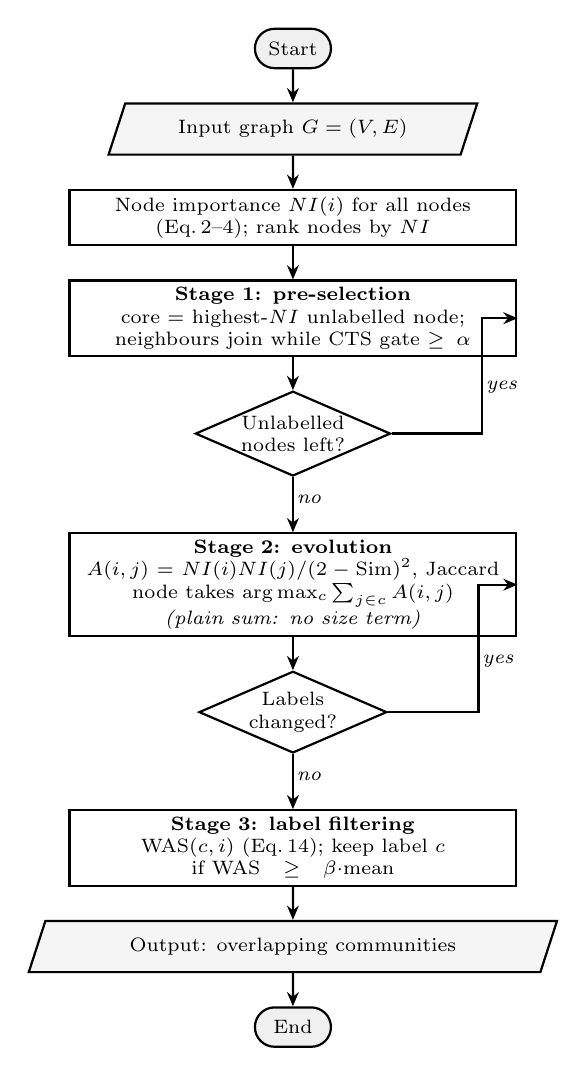
\begin{tikzpicture}[node distance=4.2mm]
\node[term] (s) {Start};
\node[io, below=of s] (in) {Input graph $G=(V,E)$};
\node[proc, below=of in, text width=55mm] (ni) {Node importance $NI(i)$ for all nodes\\(Eq.\,2--4); rank nodes by $NI$};
\node[proc, below=of ni, text width=55mm] (s1) {\textbf{Stage 1: pre-selection}\\ core = highest-$NI$ unlabelled node;\\ neighbours join while CTS gate $\ge\alpha$};
\node[dec, below=of s1] (d1) {Unlabelled\\nodes left?};
\node[proc, below=7mm of d1, text width=55mm] (s2) {\textbf{Stage 2: evolution}\\ $A(i,j)=NI(i)NI(j)/(2-\mathrm{Sim})^2$, Jaccard\\ node takes $\arg\max_c\sum_{j\in c}A(i,j)$\\ \textit{(plain sum: no size term)}};
\node[dec, below=of s2] (d2) {Labels\\changed?};
\node[proc, below=7mm of d2, text width=55mm] (s3) {\textbf{Stage 3: label filtering}\\ $\mathrm{WAS}(c,i)$ (Eq.\,14); keep label $c$\\ if $\mathrm{WAS}\ge\beta\cdot$mean};
\node[io, below=of s3] (out) {Output: overlapping communities};
\node[term, below=of out] (e) {End};
\draw[arr] (s)--(in); \draw[arr] (in)--(ni); \draw[arr] (ni)--(s1); \draw[arr] (s1)--(d1);
\draw[arr] (d1)--(s2) node[lab, pos=.4, right]{no};
\draw[arr] (d1.east) -- ++(1.15,0) |- (s1.east) node[lab, pos=.2, right]{yes};
\draw[arr] (s2)--(d2);
\draw[arr] (d2)--(s3) node[lab, pos=.4, right]{no};
\draw[arr] (d2.east) -- ++(1.15,0) |- (s2.east) node[lab, pos=.2, right]{yes};
\draw[arr] (s3)--(out); \draw[arr] (out)--(e);
\end{tikzpicture}
\caption{Architecture of the baseline TPOC-LPA~\cite{kong2026}. Symbols follow the usual flowchart convention: oval = start/end, parallelogram = input/output, rectangle = process, diamond = decision.}
\label{fig:base}
\end{figure}

\section{Diagnosis: Why Stage 2 Misbehaves}\label{sec:diag}
Eq.~\eqref{eq:stage2} adds up neighbour attractiveness without any size term. A community that grows therefore gains score for its size alone, so labels keep merging: nothing in the rule limits a community's share. We confirmed this on email-Eu (986 nodes, 42 departments, average degree 33): Stage~1 yields 335 communities at NMI 0.54, and Stage~2 then merges them all into one (NMI 0.00). On LFR graphs with realised mixing $\mu{=}0.7$ the mean NMI of the baseline is 0.05. On the opposite side, on sparse graphs such as Cora the baseline leaves 214 communities for 7 classes: the sum is too weak to merge fragments. Eq.~\eqref{eq:stage2} is the $\gamma{=}0$ end of the family
\begin{equation}
\mathrm{gain}(c)=\sum_{j\in N(i)\cap c}A(i,j)-\gamma\,\frac{s_i\,S_c}{W},\label{eq:gain}
\end{equation}
where $s_i=\sum_j A(i,j)$, $S_c=\sum_{k\in c}s_k$ and $W=\sum_i s_i$; $\gamma{=}1$ is the LPAm gain~\cite{barber2009} with node-importance weights.

\section{Proposed Modifications}\label{sec:method}
Fig.~\ref{fig:ours} shows the full pipeline and marks what we changed. Every option defaults to off, so the default code path equals Sec.~\ref{sec:base}. In the code the modifications are labelled CHANGE~1, 2, 3, 4, 6 and 9; the mapping is M1$\to$1, M2$\to$2, M3$\to$3, M4$\to$4, M5$\to$6, M6$\to$9.

\textbf{M1: triangle-based similarity.} Jaccard divides the shared neighbours by the size of the union, so two well-connected nodes in a tight community can look weakly similar. With $c$ the number of common neighbours (the triangles on edge $(i,j)$) we use $\mathrm{Sim}(i,j)=c/(1+c)$, which depends on the triangle count and not on the neighbourhood sizes. It costs a little on sparse graphs, where one shared neighbour is often chance.

\textbf{M2: best-iterate guard.} After every Stage~2 round we compute modularity (starting from the Stage~1 partition) and pass on the best round, not the last. It is a no-op unless a later round is worse, as in the email-Eu collapse.

\textbf{M3: size-corrected gain.} Stage~2 uses Eq.~\eqref{eq:gain} with $\gamma{=}1$ in place of Eq.~\eqref{eq:stage2}. On its own this fragments graphs whose labels are coarse (Karate, Dolphin, Polbooks), hence M4.

\textbf{M4: granularity rule.} Run the paper-style Stage~2 ($\gamma{=}0$) and the corrected one ($\gamma{=}1$) from the same Stage~1 partition, and keep the corrected result only if it has at most $1.5\times$ as many communities. When the two agree on scale, $\gamma{=}1$ only fine-tunes boundaries; when it shatters the graph we are in the coarse-truth case and keep the paper-style result. The test uses no labels. The threshold 1.5 was chosen by leave-one-dataset-out on our development graphs.

\textbf{M5: merge pass with a map-equation stop.} After Stage~2, communities are merged greedily by largest modularity gain $\Delta Q$ (a heap with lazy deletion). The earlier version kept all merges if the total gain passed a threshold; this wrecked SNAP-DBLP (9{,}803 communities merged into 807, NMI $0.7667\to0.6197$) because modularity rewards merging at the wrong scale. We keep the merge order but track the two-level map-equation codelength $L$ after each merge and return the prefix of merges where $L$ was lowest. If no prefix lowers $L$, nothing is merged.

\textbf{M6: boundary moves with a Synwalk score.} Nodes are visited in $NI$ order. Node $i$ moves to the neighbouring community that most increases the Synwalk objective~\cite{toth2022}
\begin{equation}
J=\sum_{m}\Big[p_{mm}\ln\frac{p_{m\to m}}{p_m}+p_{m,\neg m}\ln\frac{p_{m\not\to m}}{p_{\neg m}}\Big],\label{eq:synwalk}
\end{equation}
where for module $m$ with volume $\mathrm{vol}$ and cut $\mathrm{cut}$, $p_m=\mathrm{vol}/2|E|$, $p_{m\to m}=1-\mathrm{cut}/\mathrm{vol}$ and the other terms follow. $J$ is a sum over modules that depends only on each module's volume and cut, so a move is scored by recomputing two terms. Sweeps repeat until no node moves. There is no aggregation step: communities are never joined wholesale (a seeded Infomap collapsed LFR $\mu{=}0.7$ into one module). The whole pass is kept only if the \emph{regularised} map codelength~\cite{smiljanic2020} also falls; otherwise all moves are discarded. This gate exists because the plain map equation over-fits small graphs: a single move costs 0.16 NMI on Karate. The gate was designed after seeing that failure, so it is a post-hoc choice.

\begin{figure*}[t]
\centering
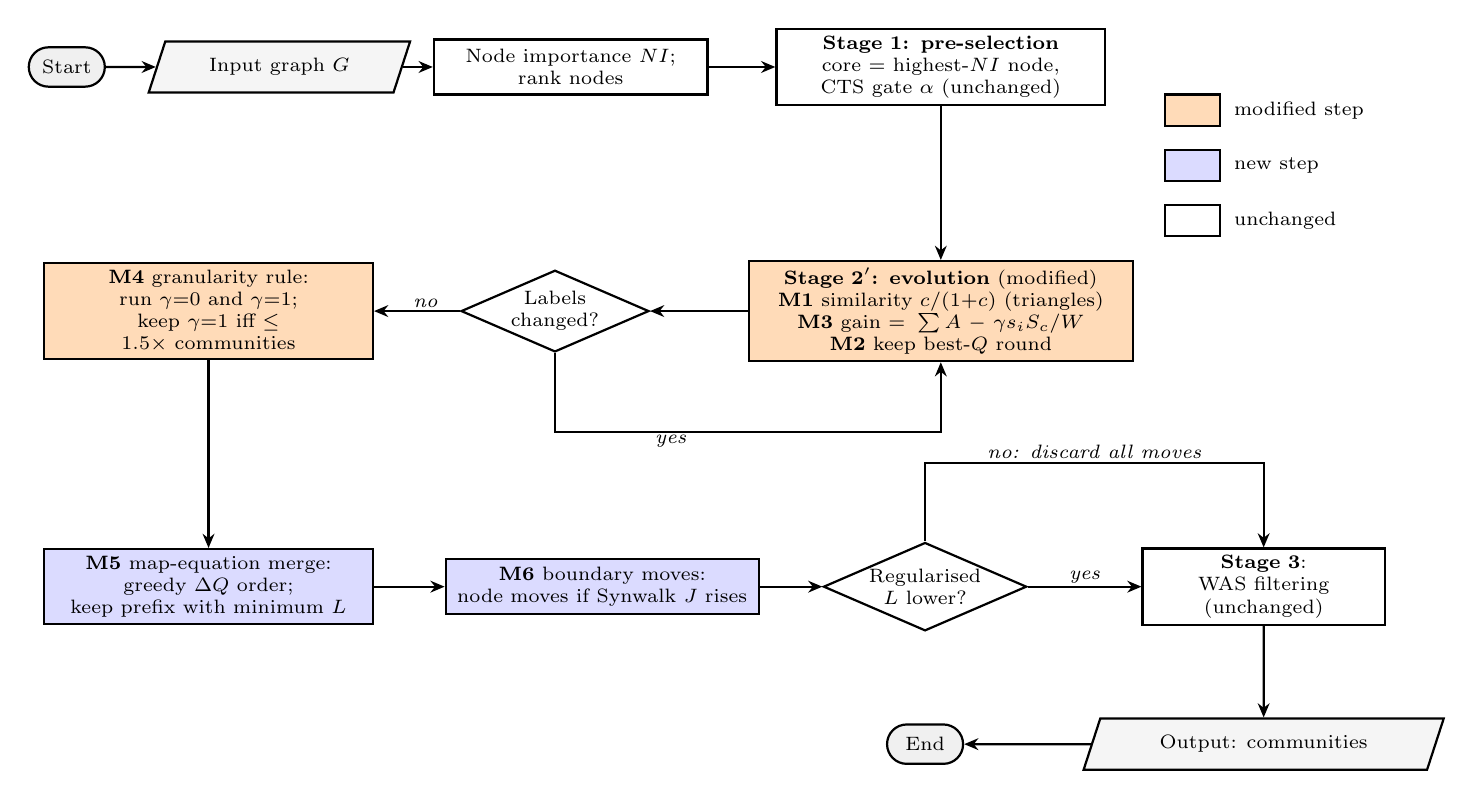
\begin{tikzpicture}[x=1cm,y=1cm]
% ---- row A: left to right
\node[term] (s) at (0.8,0) {Start};
\node[io] (in) at (3.5,0) {Input graph $G$};
\node[proc, text width=33mm] (ni) at (7.2,0) {Node importance $NI$;\\ rank nodes};
\node[proc, text width=40mm] (s1) at (11.9,0) {\textbf{Stage 1: pre-selection}\\ core = highest-$NI$ node,\\ CTS gate $\alpha$ (unchanged)};
% ---- row B: right to left
\node[modp, text width=47mm] (s2) at (11.9,-3.1) {\textbf{Stage 2$'$: evolution} (modified)\\ \textbf{M1} similarity $c/(1{+}c)$ (triangles)\\ \textbf{M3} gain $=\sum A-\gamma s_iS_c/W$\\ \textbf{M2} keep best-$Q$ round};
\node[dec] (d2) at (7.0,-3.1) {Labels\\changed?};
\node[modp, text width=40mm] (m4) at (2.6,-3.1) {\textbf{M4} granularity rule:\\ run $\gamma{=}0$ and $\gamma{=}1$;\\ keep $\gamma{=}1$ iff $\le1.5\times$ communities};
% ---- row C: left to right
\node[newp, text width=40mm] (m5) at (2.6,-6.6) {\textbf{M5} map-equation merge:\\ greedy $\Delta Q$ order;\\ keep prefix with minimum $L$};
\node[newp, text width=38mm] (m6) at (7.6,-6.6) {\textbf{M6} boundary moves:\\ node moves if Synwalk $J$ rises};
\node[dec] (g) at (11.7,-6.6) {Regularised\\$L$ lower?};
\node[proc, text width=29mm] (s3) at (16.0,-6.6) {\textbf{Stage 3}: WAS filtering\\ (unchanged)};
\node[io] (out) at (16.0,-8.6) {Output: communities};
\node[term] (e) at (11.7,-8.6) {End};
\draw[arr] (s)--(in); \draw[arr] (in)--(ni); \draw[arr] (ni)--(s1);
\draw[arr] (s1)--(s2);
\draw[arr] (s2)--(d2);
\draw[arr] (d2.south) -- ++(0,-1.0) -| (s2.south) node[lab, pos=.15, below]{yes};
\draw[arr] (d2)--(m4) node[lab, pos=.4, above]{no};
\draw[arr] (m4)--(m5);
\draw[arr] (m5)--(m6);
\draw[arr] (m6)--(g);
\draw[arr] (g)--(s3) node[lab, pos=.5, above]{yes};
\draw[arr] (g.north) -- ++(0,1.0) -| (s3.north) node[lab, pos=.25, above]{no: discard all moves};
\draw[arr] (s3)--(out); \draw[arr] (out)--(e);
% ---- legend
\node[proc, fill=orange!28, minimum width=7mm, minimum height=4mm] at (15.1,-0.55) (l1) {};
\node[font=\scriptsize, anchor=west] at (15.5,-0.55) {modified step};
\node[proc, fill=blue!14, minimum width=7mm, minimum height=4mm] at (15.1,-1.25) (l2) {};
\node[font=\scriptsize, anchor=west] at (15.5,-1.25) {new step};
\node[proc, minimum width=7mm, minimum height=4mm] at (15.1,-1.95) (l3) {};
\node[font=\scriptsize, anchor=west] at (15.5,-1.95) {unchanged};
\end{tikzpicture}
\caption{Architecture of the proposed pipeline. Orange boxes modify a step of TPOC-LPA, blue boxes are new steps, white boxes are unchanged (compare Fig.~\ref{fig:base}). Stage~1 and Stage~3 are exactly the published ones.}
\label{fig:ours}
\end{figure*}

\section{Experimental Setup}\label{sec:setup}
\textbf{Methods compared.} Fastgreedy~\cite{clauset2004}, LPA~\cite{raghavan2007}, Louvain~\cite{blondel2008} and Walktrap~\cite{pons2006} (all via the igraph C library), the baseline TPOC-LPA as we re-implemented it (TPOC$^{\dagger}$), and our pipeline M1--M6. Infomap~\cite{rosvall2008} is not in~\cite{kong2026}; we add it because M5 and M6 borrow from it, so it is the strongest reference. For overlap we compare with SLPA~\cite{xie2011}, which we implemented ($T{=}100$ iterations) and tuned the way the paper tunes it. NSA, SimCMR, WLC, UMSTMO, GREESE and MDPA have no public code that we could find, and we did not re-implement them from a paragraph of description. Their published numbers are quoted in Table~\ref{tab:paper} and are marked as such.

\textbf{Data.} \emph{Real networks:} Karate, Dolphin (group labels reconstructed from the original study), Football, Polbooks, Polblogs, email-Eu-core, Cora, Citeseer, and SNAP-Amazon, -Youtube and -DBLP~\cite{yang2012}. The SNAP graphs are our own induced subgraphs, $2.6$--$3.9\times$ larger than the subsets used in~\cite{kong2026}, with the first listed community as truth; absolute values are therefore not comparable with the paper, only across our columns. \emph{LFR:}~\cite{lfr2008} with the six settings of the paper. The generator in networkx realises a mixing far above its nominal $\mu$ (nominal 0.6 gives about 0.84), so we calibrate the nominal value until the realised mixing equals the target. \emph{Overlapping LFR:} the paper's R1--R6 (42 networks per seed, $om=2..8$) from the original generator of Lancichinetti et al., two seeds. \emph{EQ:} 12 networks of~\cite{kong2026}; we obtained 11 at the sizes in the paper (Jazz, Power, PGP from KONECT, GrQc, HepTh, Facebook, Deezer from SNAP, LastFM) and used the 2{,}708-node Cora.

\textbf{Metrics.} NMI (arithmetic normalisation) and unweighted modularity $Q$ for disjoint results; LFK-NMI, $\mathrm{NMI}_{\max}$ and the Omega index for overlapping ones; and EQ~\cite{kong2026} computed by an $O(m)$ routine that we verified against a direct $O(\sum|c|^2)$ implementation. The NMI normalisation of~\cite{kong2026} is not clear to us: for the same Fastgreedy partition of Karate it reports 0.7069 while we obtain 0.5646, and no standard variant reproduces its value. We use one metric implementation for all our columns, so only differences \emph{within} our tables are meaningful.

\textbf{Protocol.} We kept development graphs (Karate, Dolphin, Football, Polbooks, Polblogs, email-Eu, Cora, Citeseer, Amazon Photo, LFR $n{=}1000$ seeds 1--5) apart from held-out ones (72 further LFR variants, Amazon Computers, Coauthor-CS, Coauthor-Physics) and fresh ones used once. A change became a candidate default only if no held-out real graph lost more than 0.005 NMI. Several choices ($\rho{=}1.5$, the gate in M6, $\beta$) were made after looking at development data, and we list them in Sec.~\ref{sec:limits}. Stochastic baselines are averaged over 10 runs (3 on SNAP and LFR); we also computed their best run, which does not change the conclusions (mean rank on real graphs 2.4 for our pipeline, and 0.9941 against 0.9931 for Infomap on LFR).

\section{Results}\label{sec:results}
\subsection{Real networks}
@@T_REAL@@
Table~\ref{tab:real} gives the main result. The pipeline has the best mean rank (2.00 against 4.09--4.73 for every other column) and the highest mean NMI (0.7031 against 0.6585 for Infomap). Part of this margin comes from email-Eu, where the baseline collapses (0.0000) and our pipeline reaches 0.6677, above Louvain (0.5806) and Infomap (0.5873). On the three graphs shared with~\cite{kong2026} (Karate, Dolphin, Football) it scores 0.8372, 0.9495 and 0.9242, above Infomap (0.5805, 0.8993, 0.8683). On SNAP-DBLP it is marginally ahead (0.7676 against 0.7657 for LPA and 0.7631 for Infomap).

It is not best everywhere. On Cora, Fastgreedy is higher (0.4647 against 0.4192); on SNAP-Amazon, Louvain is (0.9825 against 0.9731); and on \textbf{SNAP-Youtube Infomap (0.7486) and Walktrap (0.7222) are far ahead of our 0.5745}, which is itself better than the baseline's 0.5195. We have not diagnosed this gap. Our pipeline takes 105\,s on SNAP-DBLP (93{,}432 nodes) and 67\,s on SNAP-Youtube, against a few seconds for the C implementations of the baselines.

\subsection{LFR benchmarks}
@@T_LFR@@
Table~\ref{tab:lfr} shows the mean NMI of our pipeline over the six settings is 0.9941, against 0.9905 for Infomap and 0.9805 for TPOC$^{\dagger}$. At $\mu{=}0.6$ the mean is 0.9883 against 0.9827 for Infomap and 0.9629 for TPOC$^{\dagger}$. Infomap is slightly higher on $n{=}5000$ and $n{=}10000$ at $\mu{=}0.6$ (0.9945 against 0.9940 and 0.9900 against 0.9895), which is within seed noise. The published baseline reports 0.9869 on its own $n{=}1000$, $\mu{=}0.6$ graphs; on our five graphs of that setting the baseline re-implementation reaches 0.9317 and our pipeline 0.9815. Table~\ref{tab:abl} shows where the gain comes from, and Table~\ref{tab:paper} shows the published numbers for reference.
@@T_ABL@@
\subsection{Overlapping communities}
@@T_OV@@
Table~\ref{tab:ov} reports overlap quality. With the paper's own WAS Stage~3 on top of our Stage~2, the pipeline has the highest mean LFK-NMI (0.7673 against 0.7578 for tuned SLPA and 0.7600 for TPOC$^{\dagger}$), and it wins R1--R4. It loses R5 and R6 (the 10{,}000-node families) to SLPA, and on the Omega mean SLPA is ahead (0.7571 against 0.7418). Our re-implemented baseline scores below the values published for TPOC-LPA on the same families (for instance 0.7949 against 0.8358 for R1), and we could not close that gap. We estimated what is recoverable: given our Stage~2 partition, a perfect Stage~3 would reach LFK-NMI 0.84--0.98 on R1 and R2, so most of the loss is in Stage~3; but the missing memberships are mostly nodes with a single link into the other community, and such a link is a true membership only 7--11\% of the time, so no local rule can find them.

\subsection{Extended modularity}
@@T_EQ@@
Table~\ref{tab:eq} shows that the picture for EQ is mixed. Our pipeline is best on 5 of 12 networks (Jazz, Lesmis, Power, Facebook, LastFM), SLPA with $r$ tuned by EQ itself on the other 7, and the mean EQ is 0.5920 for ours against 0.6013 for SLPA and 0.5750 for TPOC$^{\dagger}$. Our re-implemented baseline falls below its published EQ on most networks (for example Jazz 0.2848 against 0.4013, CA-GrQc 0.6966 against 0.7814); we do not know why.

@@T_PAPER@@

\section{Failed Ideas}\label{sec:neg}
We tried and dropped the following; they are kept in the code under the label ``explored, not adopted''.
\begin{itemize}
\item \emph{LLM correction of Stage~2.} A budgeted multi-select correction with local 3--8B models. Oracle headroom exists (Football $+0.059$) but a hard override with the measured accuracy of 0.817 gave NMI 0.7815 against 0.9095 structure-only.
\item \emph{Map-equation guard in place of modularity (M2).} email-Eu fell from 0.64 to 0.00, because the map equation prefers one module when structure is weak.
\item \emph{Persona (ego-splitting) Stage~3.} It matched the published overlap numbers on our design graphs and helped on held-out synthetic graphs, but lost on real graphs (SNAP-Amazon $-0.009$, SNAP-DBLP $-0.015$ ONMI against the best WAS), so we do not adopt it.
\item \emph{Near-tie and embedded-link overlap rules.} These help SNAP-DBLP only, or add nothing once WAS is applied.
\item \emph{Selecting $\alpha$ by codelength,} link-majority polishing, and consensus clustering did not pass the held-out test.
\end{itemize}

\section{Limitations}\label{sec:limits}
\begin{itemize}
\item No change is a universal improvement; all remain opt-in. Coauthor-CS and Coauthor-Physics fail our adoption rule, and the boundary moves cost up to 0.008 NMI on sparse real graphs (Cora, Citeseer, Polbooks).
\item On graphs whose labels are coarse, a modularity merge (the earlier M5) scores higher than the map-equation stop (Physics 0.4324 against 0.2790), because the resolution limit itself matches the labels. A label-free method cannot tell this case from fine-grained truth.
\item Post-hoc choices: $\rho{=}1.5$ (picked by leave-one-dataset-out on development data), the regularised gate in M6, $s{=}3$ for personas, and $\beta{=}0.8$ taken from the paper.
\item Karate remains at 0.8372 against the 1.0000 reported in~\cite{kong2026}. One node (node 8) has three links to the other faction and two to its own, so any structure-only rule assigns it the other way. We also found that networkx's Karate graph carries edge weights; unweighted, our partition has $Q=0.3715$, which equals the $Q$ reported in~\cite{kong2026}, whereas the true two-faction split has $Q=0.3582$. This suggests that the reported $Q$ and NMI do not come from the same partition, but we cannot prove it.
\item SNAP graphs and the NMI normalisation differ from those of~\cite{kong2026}; cross-paper numbers are indicative only. We could not reproduce the overlapping-LFR and EQ values of~\cite{kong2026} for our baseline implementation.
\item The overlap result rests on two generator seeds and on tuning $r$ for SLPA with the labels, which favours SLPA.
\end{itemize}

\section{Conclusion}
We re-implemented TPOC-LPA, identified an unnormalised size effect in its Stage~2, and added six opt-in modifications that keep the published behaviour as the default. Compared with baselines re-run on identical graphs, the pipeline has the best mean rank on real networks and the highest mean NMI on LFR, repairs the collapse on dense graphs, and is competitive on overlap, but it is far behind Infomap on SNAP-Youtube, behind SLPA on the largest overlapping benchmarks, and below the published EQ values. The next steps are the Youtube gap, a label-free choice of the overlap rate, and a re-run of the six baselines without public code, if their authors release it.

\begin{thebibliography}{00}
\bibitem{kong2026} Z. Kong, Y. Huo, Y. Wang and Y. Guo, ``Three-stage overlapping community detection algorithm based on label propagation,'' \emph{Expert Syst. Appl.}, vol.~317, art.~131873, 2026.
\bibitem{raghavan2007} U. N. Raghavan, R. Albert and S. Kumara, ``Near linear time algorithm to detect community structures in large-scale networks,'' \emph{Phys. Rev. E}, vol.~76, 036106, 2007.
\bibitem{barber2009} M. J. Barber and J. W. Clark, ``Detecting network communities by propagating labels under constraints,'' \emph{Phys. Rev. E}, vol.~80, 026129, 2009.
\bibitem{liu2010} X. Liu and T. Murata, ``Advanced modularity-specialized label propagation algorithm for detecting communities in networks,'' \emph{Physica A}, vol.~389, no.~7, pp.~1493--1500, 2010.
\bibitem{clauset2004} A. Clauset, M. E. J. Newman and C. Moore, ``Finding community structure in very large networks,'' \emph{Phys. Rev. E}, vol.~70, 066111, 2004.
\bibitem{blondel2008} V. D. Blondel, J.-L. Guillaume, R. Lambiotte and E. Lefebvre, ``Fast unfolding of communities in large networks,'' \emph{J. Stat. Mech.}, P10008, 2008.
\bibitem{pons2006} P. Pons and M. Latapy, ``Computing communities in large networks using random walks,'' \emph{J. Graph Algorithms Appl.}, vol.~10, no.~2, pp.~191--218, 2006.
\bibitem{rosvall2008} M. Rosvall and C. T. Bergstrom, ``Maps of random walks on complex networks reveal community structure,'' \emph{Proc. Natl. Acad. Sci. USA}, vol.~105, no.~4, pp.~1118--1123, 2008.
\bibitem{kawamoto2015} T. Kawamoto and M. Rosvall, ``Estimating the resolution limit of the map equation in community detection,'' \emph{Phys. Rev. E}, vol.~91, 012809, 2015.
\bibitem{smiljanic2020} J. Smiljani\'c, D. Edler and M. Rosvall, ``Mapping flows on sparse networks with missing links,'' \emph{Phys. Rev. E}, vol.~102, 012302, 2020.
\bibitem{toth2022} C. Toth, D. Helic and B. C. Geiger, ``Synwalk -- community detection via random walk modelling,'' \emph{Data Min. Knowl. Discov.}, vol.~36, no.~2, pp.~739--780, 2022.
\bibitem{li2020motif} P.-Z. Li, L. Huang, C.-D. Wang, J.-H. Lai and D. Huang, ``Community detection by motif-aware label propagation,'' \emph{ACM Trans. Knowl. Discov. Data}, vol.~14, no.~2, 2020.
\bibitem{xie2011} J. Xie, B. K. Szymanski and X. Liu, ``SLPA: Uncovering overlapping communities in social networks via a speaker-listener interaction dynamic process,'' in \emph{Proc. IEEE ICDM Workshops}, 2011.
\bibitem{gregory2010} S. Gregory, ``Finding overlapping communities in networks by label propagation,'' \emph{New J. Phys.}, vol.~12, 103018, 2010.
\bibitem{epasto2017} A. Epasto, S. Lattanzi and R. Paes Leme, ``Ego-splitting framework: from non-overlapping to overlapping clusters,'' in \emph{Proc. ACM KDD}, 2017.
\bibitem{lfr2008} A. Lancichinetti, S. Fortunato and F. Radicchi, ``Benchmark graphs for testing community detection algorithms,'' \emph{Phys. Rev. E}, vol.~78, 046110, 2008.
\bibitem{yang2012} J. Yang and J. Leskovec, ``Defining and evaluating network communities based on ground-truth,'' in \emph{Proc. IEEE ICDM}, 2012.
\end{thebibliography}
\end{document}
